\documentclass{article}

\usepackage{amsmath}
\usepackage{verbatim} 
\usepackage{floatflt,graphicx}
\usepackage{url}

% Default margins are too wide all the way around.  I reset them here
%\setlength{\topmargin}{-.5in}
%\setlength{\textheight}{9in}
%\setlength{\oddsidemargin}{.125in}
%\setlength{\textwidth}{6.25in}
\begin{document}

\title{GDP vs Latitude: An Exercise in Data Scraping}
\author{Lewis Fishgold}
\date{April 20, 2014}
\maketitle

There is a vast quantity of data on the web, but much of it is in a form unsuitable for direct analysis.
 The process of collecting and cleaning data from the web is called scraping. 
In this paper, I scrape and plot data from Wikipedia, in order to take a look at the tendency for countries further from the equator to be wealthier \cite{wiki-geo-wealth}.

My goal was to plot the GDP per capita (in US dollars) against the latitude of each country.
The data came from two tables: one mapping country to latitude, and another mapping country to GDP (as measured by the IMF in 2013 \cite{wiki-gdp}).
Each country covers a range of latitudes, so I took the average of the 
latitudes of the northernmost and southernmost points in each country 
 \cite{wiki-north-lat, wiki-south-lat}.

To scrape the data, I used a Python library called {\sc lxml}, which allows the use of {\sc xpath}, a formal language for querying {\sc html} and {\sc xml} documents. 
The {\sc xpath} language makes it easy to express queries such as ``get the rows of the table in the first frame with id=NavFrame''.
There were several challenges involved in parsing the latitude tables.
One was that some rows expressed information about specific lines of latitude, such as the Tropic of Cancer, rather than countries.
Another was that some cells contained extraneous links and text.
Finally, each latitude itself needed to be parsed. 
An example latitude was $23^\circ$26''21'S, and I wanted to encode this as -23.
To do so, I used regular expressions, a language for specifying patterns in strings.

To store and manipulate the cleaned data, I used a Python libary called Pandas.
After extracting the three tables, I generated a new table with the absolute value of the mean latitudes.
By taking the absolute value, I am only preserving the distance to the equator.
I then did a SQL-like join operation (called a merge in Pandas) 
on the latitude and GDP tables, 
 to yield a single table with countries, mean latitudes, and GDPs. 
 I fit a linear regression model to predict mean GDP from latitude and got an 
 $R^2$ value of 0.14, indicating that 14\% of the variation in GDP can be 
 explained by latitude.
A scatter plot of GDP vs. latitude along with the fit line can be seen in Figure \ref{fig:fig1}.

\begin{figure}[h]
\centering
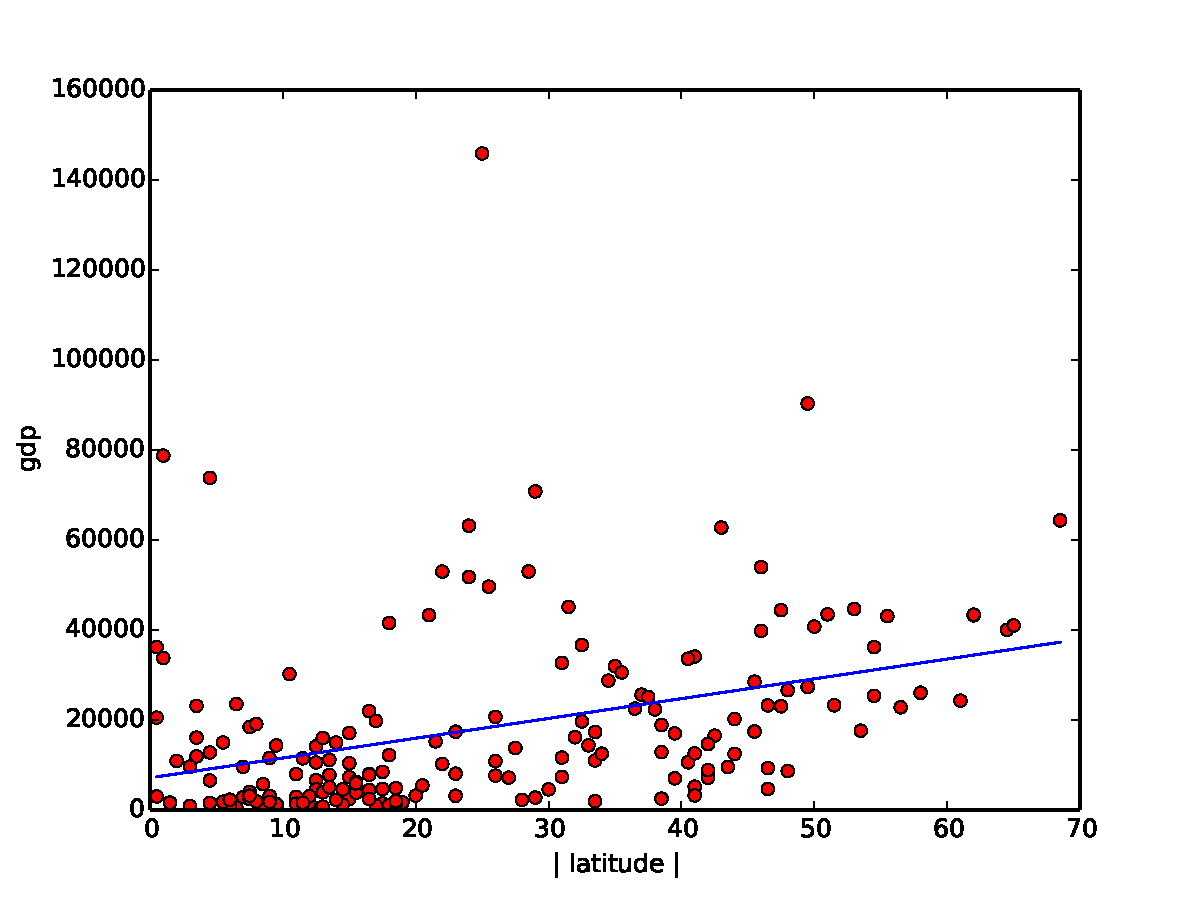
\includegraphics[scale=0.5]{scatter.pdf}
\caption{GDP per capita vs. the absolute value of the mean latitude of the countries of the world}
\label{fig:fig1}
\end{figure}

\bibliographystyle{plain}
\bibliography{document.bib}

\end{document}
